\documentclass[10pt,conference,compsocconf]{IEEEtran}

%\usepackage{times}
%\usepackage{balance}
\usepackage{url}
\usepackage{graphicx}	% For figure environment
\usepackage{color}
\usepackage{amsmath}

\pagestyle{plain}
\begin{document}
\title{Applying WaveNet on frequency data}

\author{
  Luzi Sennhauser\\
  Christoph Dehner\\
  Department of Computer Science, ETH Zurich, Switzerland
}

\maketitle

\begin{abstract}
  A critical part of scientific discovery is the
  communication of research findings to peers or the general public.
  Mastery of the process of scientific communication improves the
  visibility and impact of research. While this guide is a necessary
  tool for learning how to write in a manner suitable for publication
  at a scientific venue, it is by no means sufficient, on its own, to
  make its reader an accomplished writer. We also describe the rules
  for submission in the computational intelligence laboratory.
  This guide should be a
  starting point for further development of writing skills.
\end{abstract}

\section{Introduction}
In 2016, \cite{wavenet} introduced WaveNet, a generative model for raw audio achieving astonishing results in learning sound features and generating harmonious audio. Trained on piano music, highly dynamic piano music varying smoothly in melody, volume and speed could be generated.\\
The aim of this paper is to enhance the WaveNet architecture and apply it to a more feature-oriented representation of input data. Instead of performing a classification task on raw audio, the network is adopted to operate on the frequencies of the audio data, processed by Fouier transformation.\\
As training data in the experiments, piano samples from the MusicNet dataset, a collection of 330 freely-licenced recordings of classical music are taken. The data is publicly available online \cite{musicnet}.\\
In particular, the following topics are covered:
\begin{itemize}
\item Based on WaveNet from \cite{wavenet}, a network architecture to generate music is introduced operating on the frequencies of audio input.
\item This new network is trained and evaluated on piano music from the MusicNet dataset. Furthermore, optimization approaches as data normalization and variations in preprocessing the data are included in the experiments.
\item Results from the evaluation are analyzed in detail. In the context of the introduced network, advantages as well as weaknesses are discussed. 
\end{itemize}
The source code of the experiments can be found on GitHub.\footnote{\url{https://github.com/sennluzi/tensorflow-wavenet}}

\section{Models and Methods}
The following section describes the underlying model of the network used in the experiments of this paper. As core network the WaveNet architecture with a stack of dilated causal convolutional layers is taken. Hereupon, the data input layer is changed conceptually.
\begin{figure}[tbp]
	\centering
	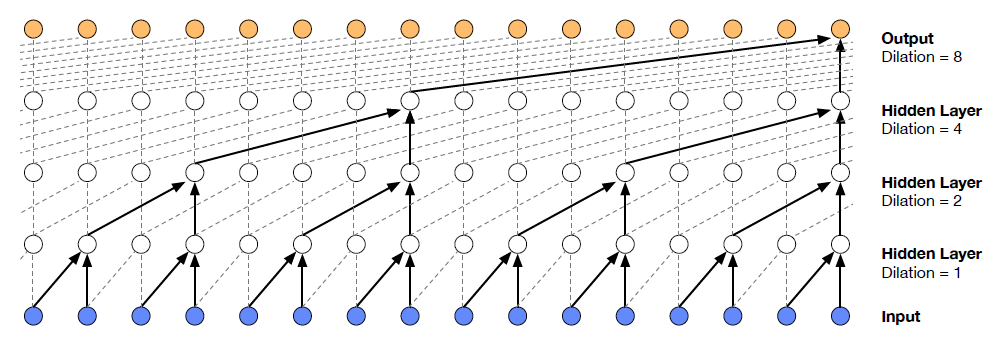
\includegraphics[width=\columnwidth]{figures/wavenet_dilated_cnn.png}
	\caption{dilated convolutional network}
	\label{fig:wavenet_dilated_cnn}
\end{figure}
\subsection{WaveNet architecture}
Given a sequence of amplitudes, WaveNet predicts the subsequent amplitude. This task is done in a classification setting: The amplitudes are quantized in 256 classes \cite{itu1988711}. The input of the WaveNet network is a sequence of such quantizied amplitudes, each encoded as a 256-dimensional one-hot vector. Performing a softmax-function in its last layer, the network outputs a probability distribution $P(x_{i+1} | x_1, ..., x_i)$ in the $i$th step. The amplitude $x_{i+1}$ of the next step is then sampled according to that distribution.\\
To model the the dependency of an audio sample on previous samples, WaveNet uses a stack of dilated convolutions. Figure \ref{fig:wavenet_dilated_cnn} depicts this architecture exemplarily for such a network of depth 4. By using exponentially growing dilations in depth, a network with $n$ dilated convolutional layers can observe the last $2^n$ input values to predict an output.\\
Training WaveNet is done similar as an autoencoder: The $i$th amplitude of the input data is predicted by only using previous input data and taken as label for the loss calculation and backpropagation. Thus, training only requires the input data and can be done in parallel. Against that, the generation of a audio sample has to be processed sequentially, since the $i$th step relies on the output of the $(i-1)$th one.\\
As a basis for WaveNet, the implementation of Igor Babuschkin is taken \cite{Babuschkin2016}. The original WaveNet paper mentions only very few coefficients for how their network is configured. Therefore reproducing the paper exactly is very hard. The following numbers are assumptions mainly based on the experience of Babuschkin's implementation. In the following experiments, the dilations are $2^n$ for $n$ taking the values $(0,1,...,8)$ and are repeated 5 times. This leads to 50 hidden dilation layers. The convolution filter size is set to $2$ and the number of channels of the residual and the dilation is $32$.\\
\subsection{Data preprocessing}
To extract frequencies, the raw audio data consisting of pressure measurements are divided into chunks of size 2048, which are then transformed into the frequency space using FFT. Therefrom, the first 150 coefficients are taken as dominant frequencies for the subsequent training. To ensure that audio features are transformed smoothly, two neighboring raw audio chunks overlap in a few samples, described by a variable $stride$. Equation \ref{eq:fft} summarized the frequency extraction of the $i^\textnormal{th}$ chunk compactly.
\begin{multline}\label{eq:fft}
\textnormal{frequencies\_coeffs}_i =
FFT(\textnormal{inputData}[i \cdot stride:\\i \cdot stride+2048])[:150]
\end{multline}
Considering real and imaginary parts of the complex Fourier coefficients separately, each chunk of 2048 raw audio samples is transformed into 300 real frequency values.\\
To decrease the dimensionality even further, principle component analysis (PCA) is used to reduce these 300 frequencies to 100 values.
These 100 PCA coefficient are considered one tone and fed into the network as one time step.\\
The eigenvectors of the PCA are shown in figure \ref{fig:pca_eigenvectors_imaginary_numbers}. Figure \ref{fig:pca_eigenvectors} illustrates how the PCA looks like when taking the absolute values of the imaginary numbers, out of which the components are built from. In this figure, one can see, that the relevant frequencies are all relatively low. Figure \ref{fig:pca_explained_variance} shows that a vast majority of the variance of the frequencies is captured by the first 100 PCA components. Summarizing, in neither of the two steps, we loose much of the original input information. This should lead to a decent compression of the audio signal.\\
To make this evident, one can figure invert all the steps and plot the compressed wave and the original wave (see \ref{fig:preprocessing_difference_waveform}). It is easy to see that they resemble a lot. After preprocessing the audio contains a cracking noise, but nevertheless is the melody and the tone of the music well audible.\\
To ensure this preprocessing still preserves the nature of the music, one can invert all steps. Although after preprocessing, there is an audible cracking, the music then is still clearly hearable and the pitches recognizable.
On one hand, the waveform looks still similar (figure \ref{fig:preprocessing_difference_waveform})
Whereas in the original WaveNet architecture, 16000 samples represented on second of audio, the adopted network only needs to process $16000/2048 \approx 8$ samples per second. However, this change infers a fundamentally different approach of audio training and generation, described in the next section. 

\begin{figure}[tbp]
  \centering
  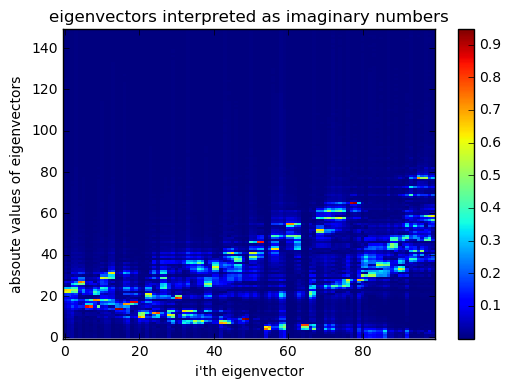
\includegraphics[width=\columnwidth]{figures/pca_eigenvectors_imaginary_numbers.png}
  \caption{Eigenvectors of the PCA where the imaginary and the real part of the FFT are stored as a separate value in the PCA component.}
  \label{fig:pca_eigenvectors_imaginary_numbers}
\end{figure}

\begin{figure}[tbp]
  \centering
  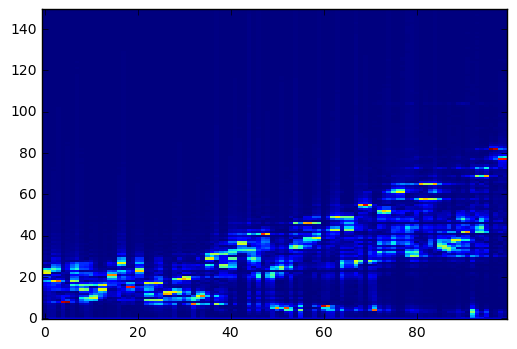
\includegraphics[width=\columnwidth]{figures/pca_eigenvectors.png}
  \caption{Transformed eigenvectors of the PCA: The values of the vectors are the absolute value of the corresponding imaginary number}
  \label{fig:pca_eigenvectors}
\end{figure}

\begin{figure}[htbp]
  \centering
  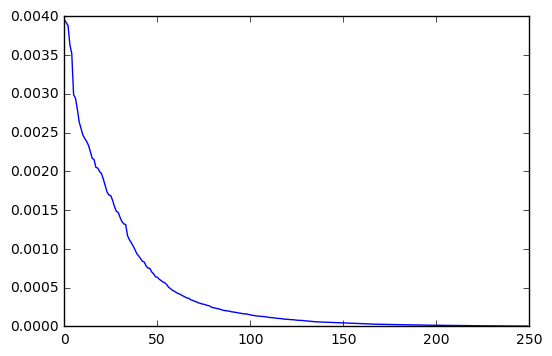
\includegraphics[width=\columnwidth]{figures/pca_explained_variance}
  \caption{Signal compression and denoising using the Daubechies wavelet basis.}
  \label{fig:pca_explained_variance}
\end{figure}

\begin{figure}[tbp]
  \centering
  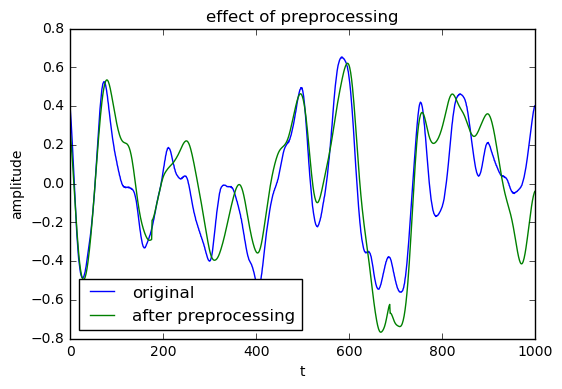
\includegraphics[width=\columnwidth]{figures/preprocessing_difference_waveform}
  \caption{An example of how the output audio differs before and after preprocessing (compression)}
  \label{fig:preprocessing_difference_waveform}
\end{figure}

\subsection{Network architecture and loss}
Whereas the original WaveNet paper designed the network to perform a classification task, the adopted network aims to train and predict the frequencies of a audio sample directly. The network input during one time step is now not only one class describing the current tone, but a 100 dimensional vector representing the frequencies of the tone of time step in a compressed way. Similarly, the output of the network is no longer a softmax layer but also a 100 dimensional vector.\\
This change in architecture also affects the loss during training. Instead of a softmax cross-entropy loss the adopted network uses the mean squared error as loss function during training.

\section{Results}
The results of all experiments are summarized in a python notebook of the GitHub repository.\footnote{"evaluate\_results.ipynb", available in the subfolder "notebooks"} Unfortunately, the adopted network could not perform as well as the original WaveNet architecture. All generated audio files stabilized on one distribution of frequencies after a few seconds. From then on the values of the frequencies did not change any more. Instead of learning the complete range of frequencies, which define the features of the audio input, the network could only learn some low basis frequencies being constantly present all the time.\\
Figures \ref{fig:original_frequencies} and \ref{fig:generated_frequencies} compare the frequencies of a recorded audio piece from the input data and the frequencies of a generated sample. In the first 200 time frames, the frequency distributions look quite similar. However, afterwards the neural network is not able to produce frequency changes continuously, while a real piece of music observes a change every 20-60 frames.\\
Furthermore the original and generated audios differ in their frequency range. Whereas the original music piece only consists of frequencies up to 32, the generated audio contains frequencies up to 105. This shows that the network has difficulties to decide which frequencies are important and cannot produce as compact and compressed audio output as it is achieved by using FFT and PCA on recorded audio data.\\
Nevertheless, the experiments of this paper can be analysed more detailled. Varying the stride and including normalization yielded conceptually different results.\\
Overlapping chunks of input data turned out to be essential for learning audio features properly. With a stride of 512 (resulting in an overlap of 75\% of neighboring data chunks) results with dynamic volume changes and frequencies within the range $[0, 105]$ within the first seconds of the generated audio could be achieved. Figure \ref{fig:generated_frequencies} visualizes the frequencies of the first 30 seconds of the output. In contrast to that, with a stride of 2048 (meaning no overlap) the network only grasped really frequencies in the range $[0,1.6]$ producing no volume or frequency dynamic in the generated audio at all.\textcolor{red}{Missing for discussion: on the one hand overlap necessary, on the other hand emphasises this to learn constant tones.}\\
A second conceptual attempt during the experiments was to normalize the PCA results before the training. The aim of this additional preprocessing task was to balance the contribution of all 100 PCA dimensions to the loss, hoping that all frequencies are learned more equally. In a first attempt, data normalzed to zero mean and unit variance turned out to produce too small loss for training. With vanishing gradients the network could not learn at all. Therefore, in a second attempt the input data was normalized to zero mean and an equal variance of all dimensions of 10. With this specifications, the network was able to learn as well as without normalization.\\
As intended, the normalization helped to learn higher frequencies. The generated results with this setting contained more different frequencies from the range $[0,360]$. But the generated audio still converged to a constant distribution of frequencies after a few seconds. 
\begin{figure}[tbp]
  \centering
  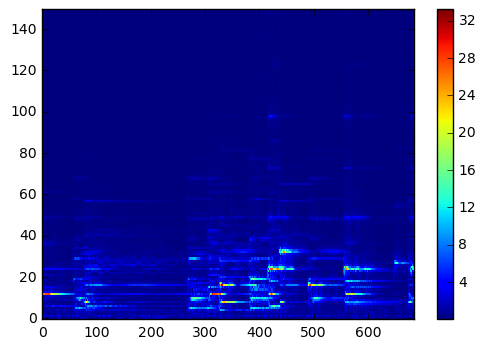
\includegraphics[width=\columnwidth]{figures/original_frequencies.png}
  \caption{Frequencies of a piano piece used for training (Recording 2322 from the MusicNet dataset). }
  \label{fig:original_frequencies}
\end{figure}
\begin{figure}[tbp]
  \centering
  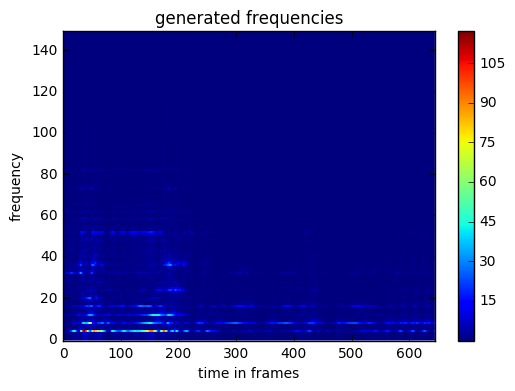
\includegraphics[width=\columnwidth]{figures/generated_frequencies_20s_2.png}
  \caption{Frequencies of a generated audio piece, model trained on the MusicNet dataset with $stride=512$ and no normalization.}
  \label{fig:generated_frequencies}
\end{figure}

%\begin{figure*}[tbp]
%  \centering
%  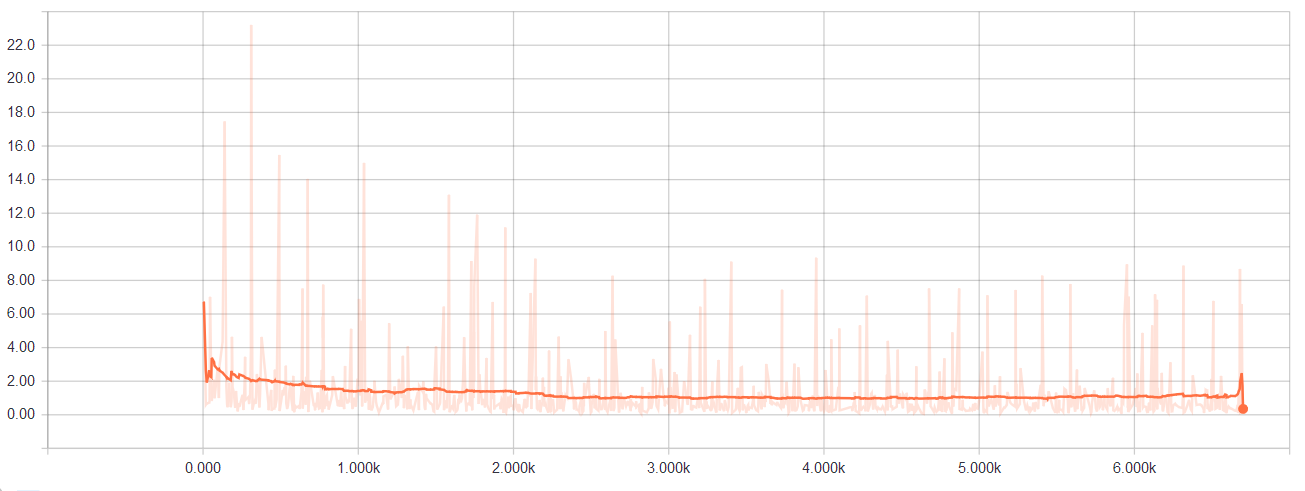
\includegraphics[width=\textwidth]{figures/loss.png}
%  \caption{Training error}
%  \label{fig:training_error}
%\end{figure*}

\section{Discussion}
The approach of this paper could be promising due to the following reason: The original WaveNet paper's network has to learn the behaviour of sound consisting of repetitive oscillations. With transforming the signal to the Fourier space, we take this burden from the neural network. The network can focus on data which is more related to the final tone. For example while a tone is the same for a certain time, the output of the network is also the same.\\
But it might be exactly this phenomenon which makes good music generation impossible. During training, the network might do really well only staying on one and the same pitch, because changes happen in too rare occasions to influence the overall loss.\\
Future work based on that paper, one could try to include the rate of changing tones into the loss function and to punish a network when producing too many times in a row a similar output.\\
There are two reasons one could think of, why this approach's result does not match its expectations:
\begin{itemize}
  \item The original paper quantizes the amplitudes and can then use a softmax layer as a last layer of the network. In this new approach, we need continous values (PCA coefficients). Since the results are much worse than with WaveNet, the missing quantization (and connected to it the missing softmax layer) might be the reason behind this phenomenon.
  \item The original WaveNet has a probability distribution as output. The exact amplitudes are then sampled according to that distribution. In the approach presented in this paper, one relies on continuous values, which are directly calculated (no probabilities included). In future work, one can change the model to produce a probability distribution of the output values.
\end{itemize}

\section{Summary}
With WaveNet an already very promising music generation network is presented. It relies on predicting amplitudes when the preceeding amplitudes are given. In this paper it is investigated whether transforming the data to the Fourier space improves the predictions. After transforming, the dimensionality of the audio file is vastly diminished. But at the same time, the ability to quantize the network's outputs is lost. Unfortunately the network returned results not as good as with the original WaveNet paper. With the new method, the generated audio files rapidly converge to one steady tone. The changing behaviour of pitches is not learned by the network.

\bibliographystyle{IEEEtran}
\bibliography{paper}
\end{document}
